\section{Intuitive Data Collection}

\subsection{Measurement}
\begin{objectives}
    \item Learn existence of uncertainty
    \item Know difference of precise and accurate
    \item Know how to do error propagation
    \item Learn different data type
    \item Understand degree of freedom
    \item Distinguish first and second hand data and tell if we can trust it
\end{objectives}
\subsubsection{Uncertainty}
 No data is absolutely correct because of many reasons.So how do we measure the uncertainty of a data? 
 \begin{description} 
    \item[Precision]: How similar to other observation.
    \item[Accuracy]: How close to the accepted value.\\
    \begin{examplebox}{Accuracy}
    A stopped clock is very precise because its readings are exactly the same. It is not accurate because its readings are not the right time.
    \end{examplebox}
    
    \item[Reading Units]: cm,mm,m,etc.
 Smaller reading units mean more precise.   \item[Significant Figures]:any digit of a number that is known with certainty.\\
 \begin{examplebox}{Significant Figures}
 \(5 \times 10^2\)is less precise than \(5.00 \times 10^2\) because it has fewer significant numbers.
 \end{examplebox}
  
    \item[Decimal Place]: the position of a digit after the decimal point, each successive position to the right having a denominator of an increased power of ten.
    \item[Dimensionless]: when a quantity has no unit.
\end{description}


\subsubsection{Error Propagation}
\textbf{:How do we measure Uncertainty?}\\

\textbf{Uncertainty} can be represented by \( x \pm \triangle x \), where \(\triangle x\) is called the \textbf{Absolute Error}.It can also be represented by \( \frac {\triangle x}{x} \times 100 \% \)  which is the \textbf{Relative/Comparative Error}.\\

\begin{examplebox}{Error}
\(9.5 \pm 0.5 cm\) absolute error is \(\pm 0.5 cm\), relative error is \(\frac{0.5 cm}{9.5 cm} \times 100 \% = 5.263 \% \).
\end{examplebox}
\vspace{0.5cm}

For a value which is the result of math operation of some uncertain data, \textbf{error and uncertainty can only become larger}.\\ We can use \textbf{Differential Infinitesimal} to attain the uncertainty of the result of any operation of the data. \\

\begin{examplebox}{Differential Infinitesimal}
For \( \times and \div \), Absolute Error add. For \( + and - \), Relative Error add.\\ Let \(z=x+y\) or \(z=x-y\), then \(dz=dx=dy\), so \(\triangle z=\triangle x+\triangle y\), note that the minus is turn into plus because error can only become larger.\\ Let \(z=xy\) or \(z=\frac{x}{y}\), do differentiation \(dz=ydx+xdy\), then divide it by xy \(\frac{dz}{xy}=\frac{ydx}{xy} \frac{xdy}{xy}\), so \(\frac{dz}{z}=\frac{dx}{x} +\frac{dy}{y}\), which is \(\frac{\triangle z}{z}=\frac{\triangle x}{x} +\frac{\triangle y}{y}\).
\end{examplebox}

\subsubsection{Data Type}: Data can be sorted to different categories as well.
\begin{itemize}
    \item \Index{Qualitative Data} A.K.A. \Index{Categorical Data}: If the individual observations are categorical responses.
    \begin{itemize}
        \item \textbf{Nominal}: Only categories matters, nothing to do with order. \\
        \begin{examplebox}{Nominal}
        gender, color, blood type
        \end{examplebox}
        
        \item \textbf{Ordinal}: Order matters. It can be sorted. \\
        \begin{examplebox}{Ordinal}
        10th, 11th, 12th; Jan, Feb, Mar...
        \end{examplebox}
    \end{itemize}
    \item \textbf{Quantitative/Numerical Data}: If each observation is a number.
    \begin{itemize}
        \item \textbf{Discrete}: If the possible values of the variable correspond to isolated points on the number line.
        \item \textbf{Continuous}: If the set of possible values forms an entire interval on the number line.
        \begin{itemize}
            \item \textbf{Ratio}: The distinction with Interval is that zero0 means absence of something. ex) Kelvin degree(0-no heat)
            \item \textbf{Interval}: ex) $0\textasciitilde 10$ grade
, 0 does not mean that no work is done.        \end{itemize}
    \end{itemize}
\end{itemize}

\subsubsection{Degrees of Freedom}
 \begin{description} 
    \item[Degrees of Freedom]: Number of independent observations. Observations should be independent from each other, because dependent ones have bias. 
 \end{description} 
 If other values $x_1 to x_(n-1)$are given and the Ari-thematic Mean value $\bar x$is also given, it's easy to calculate out $x_n$, but then the degree of freedom would be $n-1$ since $x_n$ is dependent. 
 \subsubsection{First V.S. Second Hand Data}
 \begin{description} 
    \item[First Hand Data]: Myself did the study and got this data. It's very credible to me.
    \item[Second Hand Data]: Other did the study and I can only use it. Some of them are credible, some of them are garbage.
 \end{description} 
 \begin{Question}
    How much can I trust some Second hand Data? 
 \solution \begin{enumerate}
    \item Who collect it? Is the institution capable of doing the study? \item Author of the paper? Is it authentic? 
    \item Institution behind it? 
    \item Reference? Original data can be very different to what you see now. 
    \item Purpose? Why and how the data is collected? Any bias?
\end{enumerate}
 \end{Question}


\vfill
\newpage

\subsection{Sampling and Surveys}
To do research, the first step is to \textbf{collect data}. To attain creditable and reliable data, it's crucial for researchers to select samples from a population in the correct ways.
\\
\begin{objectives}
    \item Learn different Sampling Methods
    \item Know advantages and drawbacks of each sampling method
    \item Learn different approach of Survey how it is conducted
    \item Understand bias and how it is created
    \item Learn ways to eliminate bias
\end{objectives}

\subsubsection{Sampling Methods}  To learn about a population, it is impossible to study every individual in the population, so researchers only select some individuals from the population to focus on and infer information about the population using data collected. The following are the common methods of drawing samples from the population.
\begin{description}
    \item [Simple Random Sampling]:Fast, easy, every individual has the same chance of being selected. It is so useful because it can \textcolor{red}{reduce the effect of possible confounding variables}.  
    \item [Stratified Sampling]: Entire population is divided to different groups based on characteristics, then choose randomly from each group.The purpose of choosing from all groups is to becoming as \textcolor{red}{representative to the entire population as possible}.   
    \item [Quota]: One special kind of Stratified sampling which sample size is based on the \textcolor{red}{ratio of individuals of different group}.
    \item [Cluster Sampling]: Withing the population, there are naturally \textcolor{red}{existed groups which are already very representative of the population}. Choose a group as sample simply is easy and fast.
    \item [Systematical Sampling]: Randomly assign a characteristic which has nothing to do with the study.and \textcolor{red}{all individuals with this characteristic are selected}. Every individual has zero or one hundred percent possibility to be chosen. For example, all students in blue are chosen to a study about math.
 \end{description} 
 
 \subsubsection{Different Approach Of Survey}
A survey is to directly ask people questions and collect all answers.There are some different methods of doing a survey with various advantages.
\Index{Questionnaire},Question for people to answer and return. It can be conducted through Mail(Email), Group, Drop-Off.
\Index{Interview}, Researchers ask people questions one by one and record the answer. It can be conducted{Phone, Face to Face}.
\Index{Poll},One question Questionnaire. It can be conducted through Phone, Face to Face, Internet.

 
 \subsubsection{Types of Bias}
 If the sampling methods researchers use are incorrect or the study is bad designed, then the data of the study is unreliable because bias exists.\\
 
 
\Index{Bias}: The tendency for samples to differ form the corresponding population in some systematic way.
    \begin{description}
       \item[Selection Bias]: The selection of subjects is biased. 
       \begin{enumerate}
           \item \Index{Non-Response Bias}: When some of the subjects do not response, and they have meaningful difference from the respondents.\\To reduce it: Engage in conversation prior to the survey.
            \item \Index{Under-Coverage} : When the subjects are not enough to represent the entire population.\\ \textcolor{red}{To reduce it:Use proper Sampling Method, increasing sample size cannot reduce it.}
            \item \Index{Self-Selection} : Voluntary selection. The result over-represents people with certain opinion.\\ \textcolor{red}{To reduce it:Make people engage in it. Change approach of the survey to give opportunity to other respondents.}
       \end{enumerate}
            
      
       \item[Respondent Bias]: The subjects cause the bias.
       
       \begin{enumerate}
      
           \item \Index{Extreme-Responding} : The respondents only choose the top answers(very agree, very disagree).
           \item \Index{Yea-Nay saying} : The respondents always say Yes or No to avoid embarrassment or lie.
           \item \Index{Social Desirability} : The respondents in the way they think is correct.\\\textcolor{red}{To reduce it:Forced-choice options; Proxy-Subjects--Interview a close person instead of the actual person; Bogus-Pipeline--Make people believe you can tell if they are honest or not; Selection Interviewers-- Let the subjects choose who to interview them; Self-Administered Questionnaires-- Let the subjects answer on their own; Randomized-Response Technique--Make the subjects believe that the researchers do not know who answers which question.}
       \end{enumerate}
       
       \item[Researcher Bias]: The researchers cause the bias.
       \begin{enumerate}
   
            \item \Index{Leading Question} : The wording of the question leads the respondents to answer in a certain way.
            \item \Index{Misleading Question} : The questions are not clear to understand its intention.\\ \textcolor{red}{To reduce it: Use clear language with appropriate options.}
            \item \Index{Reporting Bias} : The reporter under-report unexpected or unwanted results by attributing them to measurement error.\\ \textcolor{red}{To reduce it:Double Blind.}
            \item \Index{Procedural Bias} : When unfair pressure is applied to the subjects to make them answer quickly.\\ \textcolor{red}{To reduce it: Improve experiment design so that subjects have enough time; Random order questions.}
       \end{enumerate}
    \end{description}
\
\subsubsection{Experimental Error}
Most experiments have some error in them. Some error is inevitable but some can be avoided.
\begin{description}
    \item[Reading Error]:\( x\pm \triangle x \) It is from measurement, and exists in all data. It is associated with Instruments' maximum precision, \( \triangle x \) is half the smallest reading unit for \textbf{Analog Instrument} and full smallest reading unit for \textbf{Digital Instrument}. It creates No Bias.
    \item[Random Error]: It is due to \Index{Sampling Variability}. Variability naturally exists, and can not be removed. Standard Deviation can measure it. It creates No Bias.
    \item[Systematical Error]: It comes from wrong set up and wrong use of instruments or lack of skills. Somehow our performances in measurement pushes all observations to one direction. It creates Bias.\\ Depending on the stage the bias happens in, it can be classified as:
\begin{description}
    \item[Pre-trial Bias](Design)
    \begin{enumerate}
        \item \textbf{Selection Bias}: When we decide whether individuals are suitable for the experiment, according to some desired characteristics(Exclusion Criteria). If the criteria is not clear enough, then bias will happen.
        \item \textbf{Channeling Bias}: It is due to a Risk Factor, it's impossible to randomly assign subjects to groups(children and old).
        
    \end{enumerate}
    \item[Trial Bias](measurement, treatment)
    \begin{enumerate}
        \item \textbf{Chronological Bias}: During the period of experiment, technology might change, new discoveries made, researchers become more skilled and experienced. (We can use Block to eliminate the effect).
        \item \textbf{Interviewer Bias}: Interviewers use Leading Question to gather Data(some factors they know in advance can effect the result).
        \item \textbf{Recall Bias}: When the information is hard to obtain from measurements, and we have to rely on subject accounts, it could happen that the subjects created an association between unrelated things in their minds.
        \item \textbf{Survivors-hip Bias}: n people to begin with and m people at the end. Subjects disappear during treatment.
        \item \textbf{Transfer Bias}: Follow up measurement after treatment, some subjects do not wish to participate (especially clinical).
        \item \textbf{Misclassification}: Reporters write down the wrong treatment level or type during treatment; wrong classification as success or failure or not clear definition fro success and failure.
        \item \textbf{Performance}: Groups receive slightly different condition that should be identical(confounding variable). Variability between Researchers and within various instances for the same researchers.
        
    \end{enumerate}
    \item[Post-trial Bias](conclusion, analysis)
    \begin{enumerate}
        \item \textbf{Reporting Bias}: Not all experiment results are published, positive results are easier to be published.
        \item \textbf{Confounding Bias}: It can cause wrong Cause-effect relationship.
    \end{enumerate}
\end{description}
    
\end{description}

\begin{Question}
What is the difference between cluster and stratified sampling?
\solution For a cluster, it has variability naturally. For a strata, it has the same characteristics.
\end{Question}
\begin{Question}
How is systematical sampling possibly biased?
\solution Because probably the I may choose the samples with a certain characteristic that affect the response variable.
\end{Question}
\begin{Question}
What is drop-off?
\solution It means that the researcher give the subject questionnaire and than leave them alone to finish it.
\end{Question}
\begin{Question}
Why would Extreme-Responding exist?
\solution Because people do not want to carefully answer it.
\end{Question}




    
\subsection{Experimental Design}
There are several ways to gain data in a research, including \textbf{Direct Measurement, Survey and Experiment}
\\ A well-designed experiment requires more than just manipulating the explanatory variable;  the design has to eliminate the effect of other possible variables.\\
\begin{objectives}
    \item Distinguish between observation and experiment study
    \item Learn important terms in experimental design
    \item Understand key concepts in experimental design
    \item Know different design methods
\end{objectives}
\subsubsection{Observational V.S. Experimental Study}
Study can also be sorted to two different type. They have different design and different conclusions can be drown from the data. 
\begin{description}
    \item[Observation]: The researchers observe characteristics of a sample selected from populations. Its goal is to draw conclusion about the population. Result in Coloration, some can be ridiculous.
  
    \item[Experiment]: The researchers observe how a response variable behaves if the explanatory variable is manipulated. Its goal is to draw conclusion about the explanatory variables' effect. Result in cause-effect relationship.
    \begin{description}
    \item[Response Variable]: Dependent variable, which we measure.
    \item[Explanatory Variable]: Independent variable, which we control.
    \item[Factor]: Other factors need to be controlled or the result is not correct because they can also affect the response variable as well as the explanatory variable.   
    \begin{itemize}
        \item \textbf{Confounding Variable}: Logical possible affecting variable.\\
  \begin{examplebox}{Confounding Variable}
  If we study different math teachers' effect on math scores of high-school students, IQ would be a quite important Confounding Variable which we have to control.  
  \end{examplebox}
   
  \item \textbf{Lurking Variable}: We don't even know they exist, but they are actually out there affecting the result.
    \end{itemize}
    \end{description}
    \end{description}
    


\subsubsection{Key Concepts in Experimental Design}
\begin{description}
    \item[Random Assignment]: Random assignment of subjects to treatment and of treatment to trial to ensure that the experiment does not systematically favor on experimental condition over the other. It is very powerful in eliminating other \textbf{lurking variables}.
    \item[Blocking]: Using extraneous variables to create groups(blocks) that are similar. All experimental conditions are then tried in each block. By changing the level of the confounding variables and doing  the experiment again and again, the effect of them can be eliminated or understood.
    \item[Direct Control]: Holding the confounding variables constant during each treatment so that their effect cannot confound with those of the factors of interest.
    \item[Replication]: Ensuring that there is an adequate number of observation for each experiment to be reliable.
    \item[Control Group]: Most experiments compare a group that receives a particular treatment to a \textbf{Control Group} that receives NO treatment to test the effectiveness of this treatment. The one which receives the treatment is called \textbf{Experimental Group}.
    \item[Positive Control]: One treatment is already tested and proven to be effective. It is used to compare the the factor of interest in order to see the improvement of effectiveness.
\end{description}
In some experiments, psychology of the \textbf{subjects and observers} is really powerful and effects the experiment results. \\
\begin{examplebox}{psychological effect}
For example,for the subjects, it the researchers tell them they are tasting the most decent and expensive wine in the world even though the wine is in fact very cheap, most subjects would make such a comment that the wine is just the best they've ever drunk; they probably are not lying because the power of believing can really make difference. For observers, if they are testing the effectiveness of a new drug they invent, they may or may not intentionally measure the effectiveness higher to make more funding.(Measurement bias)
\end{examplebox}
\vbox{}
There are ways to eliminate these effects.
\begin{description}
    \item[Placebo]: Something feels identical to the real treatment but does not work at all. ex) drug and a candy looks the same
    \item[Single Blind]: The subjects do not know which treatment they receive but the observers do know. or vice versa
    \item[Double Blind]: Neither the subjects nor the observers know which treatment is received by each subject.
\end{description}
\subsubsection{Experiments Design}
It includes some different experimental designs with various advantages and drawbacks.


\begin{center}
    \Index{One Shot}
\end{center}
It is used to see if there is any of the expected effect at all. There might be too many Lurking Variable.\\Select Group $\rightarrow$ Administer Treatment $\rightarrow$ Observe
\vspace{3ex}
\begin{center}
    \Index{One-Group Pre-Post}
\end{center}
It offers a starting point to see if the treatment is effective. The selection is not random, so there might be bias.\\ Select $\rightarrow$ Observe $\rightarrow$ Treatment $\rightarrow$ Observe $\rightarrow$ Compare
\vspace{3ex}
\begin{center}
    \Index{Static Group}
\end{center}
With a control group and an experiment group, we can observe them at the same time. It is used to test rival hypothesis--would it still works without the treatment and if the effect really associates with the factor of interest. However it only works if the groups are comparable at the beginning(No significant difference that can affecting the result)\\ Select $\rightarrow$ Treatment $\rightarrow$ Observe $\rightarrow$ compare\\Select $\rightarrow$ Treatment $\rightarrow$ Observe $\rightarrow$ compare
\vspace{3ex}
\begin{center}
    \Index{Randomly selected Control Group}
\end{center}
Random selection is very powerful on eliminating lurking variable.
\vspace{3ex}
\begin{center}
    \Index{Simple Block Design}
\end{center}
Identify the confounding variable and keep it at the same level while we run the experiment for all levels of the factor of interest.
\vspace{3ex}
\begin{center}
    \Index{Factor Design}
\end{center}
We change the level of the confounding variables and run the experiment again, till we have all the combinations of all the levels of confounding variables and factor of interest.
\vspace{3ex}
\begin{center}
    \Index{Latin Square}
\end{center}
Changing the the levels of confounding variables can be super redundant because for 3 factors with K1 K2 K3 level, we have to do \(K1*K3*K2\) combinations. So we have \textbf{Latin Square}, which is only 9 times, so much less work, but the disadvantage is that all factors have to have the same number of levels to work.
    \begin{figure}[H]
        \centering
        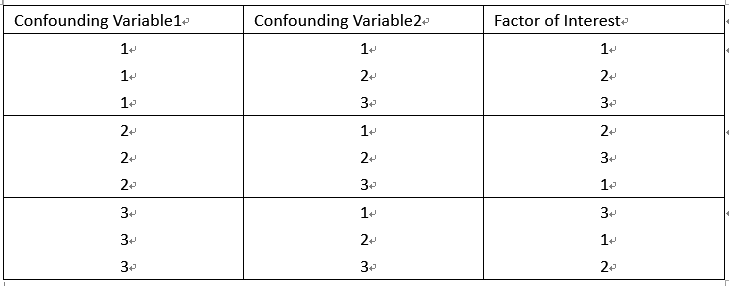
\includegraphics[width=15cm]{cf.png}
        \caption{Latin Square}
        \label{fig:my_label}
    \end{figure}
\vspace{3ex}
\begin{center}
    \Index{Solomon-four Group}
\end{center}
to reduce the effect of pre-post studies on the true measurement after the treatment, we introduce \textbf{Solomon-four Group}.In this method, subjects are randomly assigned to four groups.\\
    Random Select $\rightarrow$ Observe $\rightarrow$ Treat $\rightarrow$ Observe\\Random Select $\rightarrow$ Observe  $\rightarrow$ Observe\\Random Select  $\rightarrow$ Treat $\rightarrow$ Observe\\Random Select  $\rightarrow$ Observe
\vspace{3ex}
\begin{center}
    \Index{Counter Balancing}
\end{center}
It can average the effect of subjects' difference, by giving each subject all the levels of treatment. Each subject is treated with all treatments.

\vfill
\newpage


                                                                                                                                                                                                                                                                                                                                                                                                                                                                                                                                                                                                                                                                                                  